\begin{frame}[allowframebreaks]{DreamBooth}
\begin{figure}
    \centering
    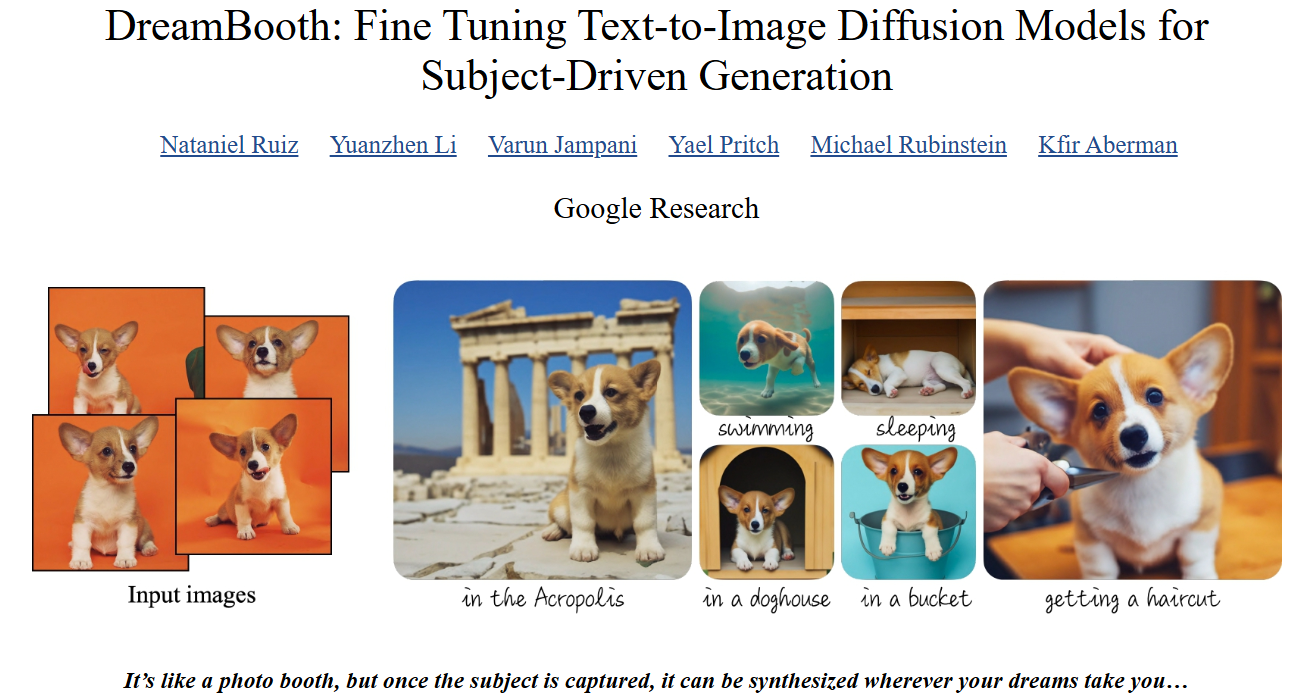
\includegraphics[width=\linewidth,height=\textheight,keepaspectratio]{images/adv-img-gen/dreambooth-1.png}
\end{figure}

\framebreak
\textbf{What is DreamBooth?}
\begin{itemize}
    \item A method for fine-tuning large diffusion models on a small number of images.
    \item Developed by Google Research (2022).
    \item Allows personalization of generative models with minimal data.
\end{itemize}

\framebreak
\textbf{Key Concepts}
\begin{itemize}
    \item \textbf{Personalization:} Adapts a pre-trained model to generate images of specific subjects (e.g., pets, people).
    \item \textbf{Fine-tuning:} Uses a small set of images to adjust the model's parameters.
    \item \textbf{Text Conditioning:} Leverages text prompts to guide image generation.
\end{itemize}

\framebreak

\begin{figure}
    \centering
    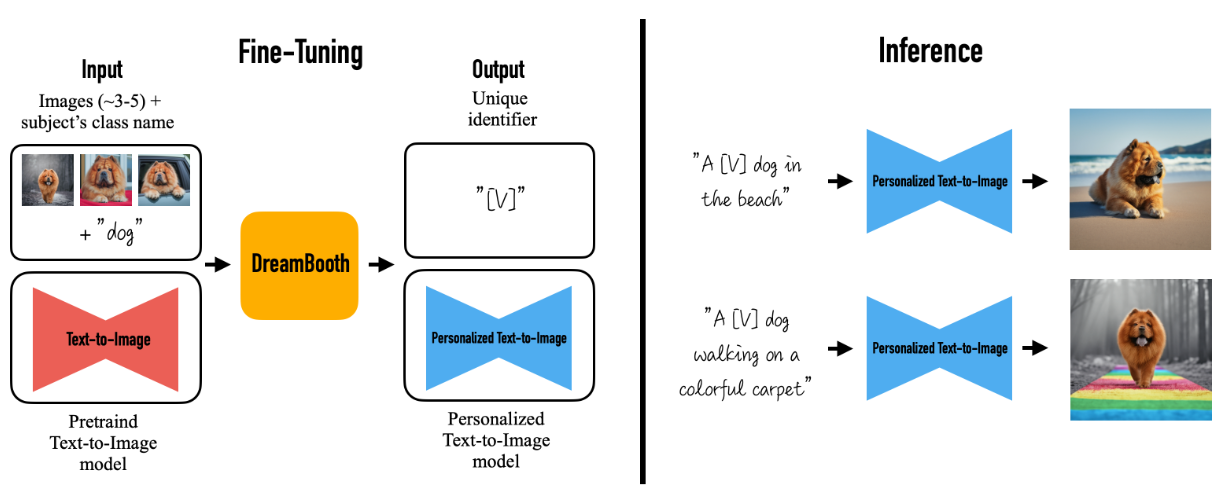
\includegraphics[width=\linewidth,height=\textheight,keepaspectratio]{images/adv-img-gen/dreambooth-2.png}
\end{figure}

\framebreak

\textbf{How Does DreamBooth Personalize Models?}
\begin{itemize}
    \item DreamBooth teaches a model to recognize a new subject using just a few photos.
    \item After training, the model can create new images of that subject in different places or situations.
    \item This is called ``few-shot'' learning—using only a few examples!
\end{itemize}

\framebreak
\begin{figure}
    \centering
    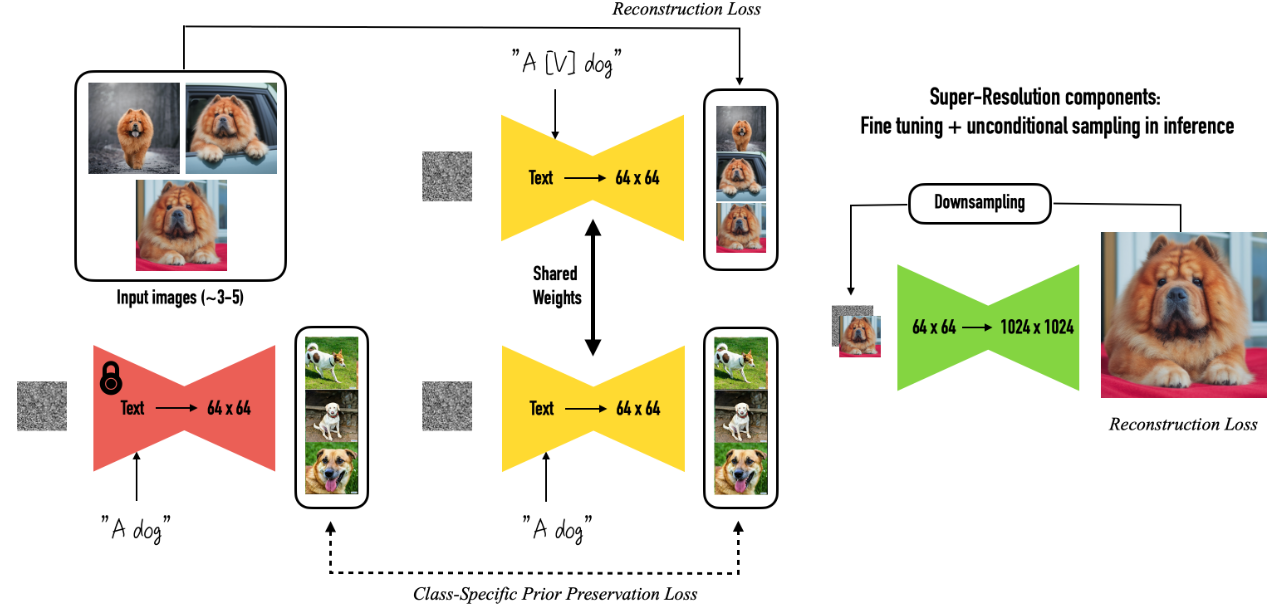
\includegraphics[width=\linewidth,height=\textheight,keepaspectratio]{images/adv-img-gen/dreambooth-3.png}
\end{figure}

\framebreak

\textbf{How Do We Tell the Model About the New Subject?}
\begin{itemize}
    \item We use a special made-up word (called a \textit{rare-token}) to represent the new subject.
    \item For example: ``a photo of \texttt{sks dog} at the beach''.
    \item The model learns to link this rare-token to the subject in your photos.
\end{itemize}

\framebreak

\textbf{Why Use Rare-tokens?}
\begin{itemize}
    \item Rare-tokens are unique and not found in the model's original training data.
    \item This avoids mixing up your subject with things the model already knows.
\end{itemize}

\framebreak

\textbf{How Does DreamBooth Avoid Forgetting?}
\begin{itemize}
    \item If we only train on your subject, the model might forget how to make other images.
    \item To prevent this, we also show it regular class prompts (like ``a photo of a dog'').
    \item We use a special loss to balance learning the new subject and keeping old knowledge:
    \[
        \mathcal{L}_{\text{total}} = \mathcal{L}_{\text{subject}} + \lambda \mathcal{L}_{\text{prior}}
    \]
    where:
    \begin{itemize}
        \item $\mathcal{L}_{\text{subject}}$ = loss for your subject (rare-token prompt)
        \item $\mathcal{L}_{\text{prior}}$ = loss for general class (class prompt)
        \item $\lambda$ = weight to balance the two
    \end{itemize}
\end{itemize}
\end{frame}

\begin{frame}[allowframebreaks]{DreamBooth: Results}
\begin{figure}
    \centering
    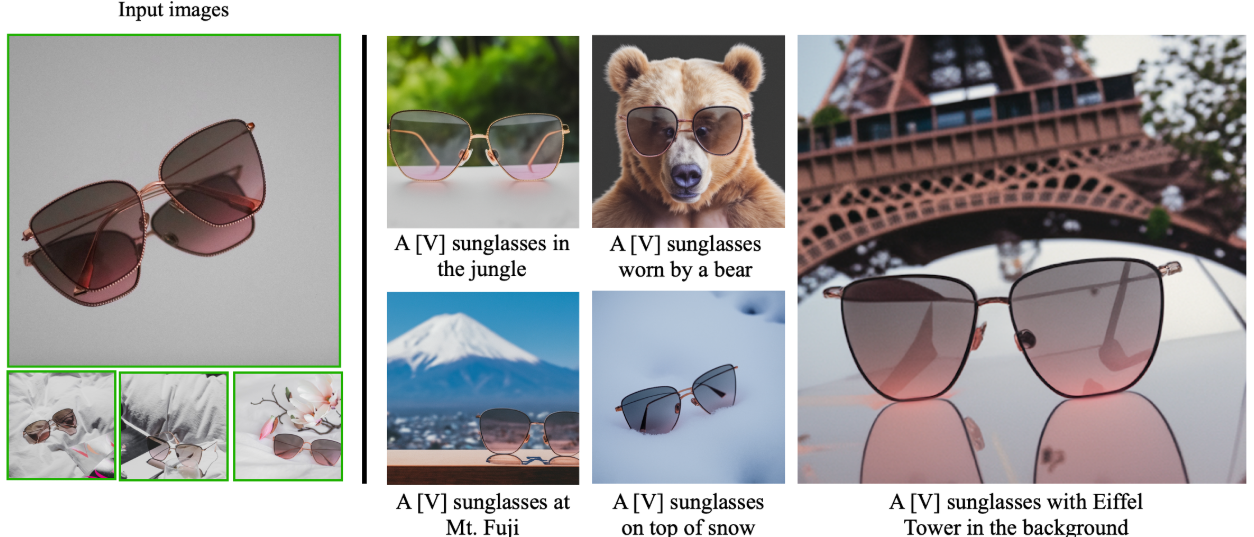
\includegraphics[width=\linewidth,height=\textheight,keepaspectratio]{images/adv-img-gen/dreambooth-result-1.png}
    \small [Ruiz et al., 2023](https://arxiv.org/abs/2208.12242)
\end{figure}

\framebreak

\begin{figure}
    \centering
    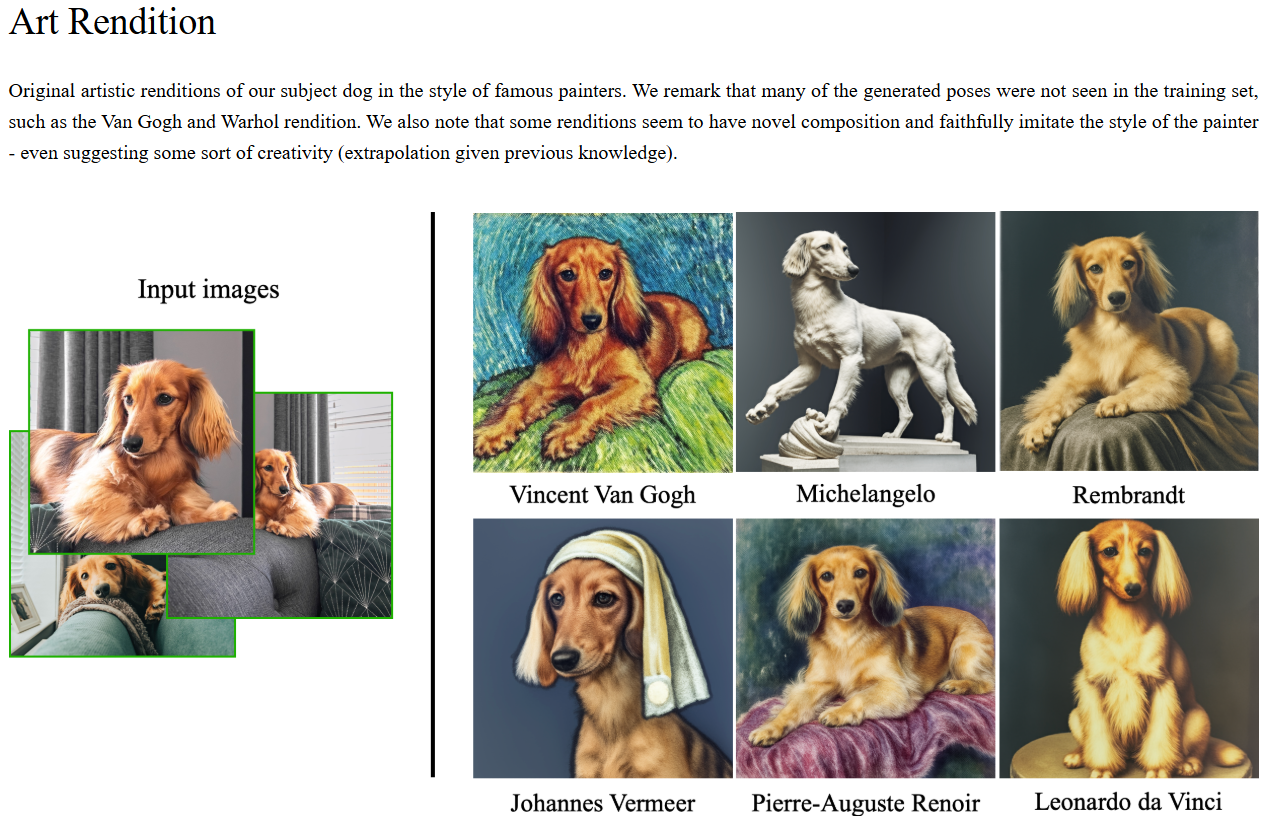
\includegraphics[width=\linewidth,height=\textheight,keepaspectratio]{images/adv-img-gen/dreambooth-result-2.png}
    \small [Ruiz et al., 2023](https://arxiv.org/abs/2208.12242)
\end{figure}

\framebreak
\begin{figure}
    \centering
    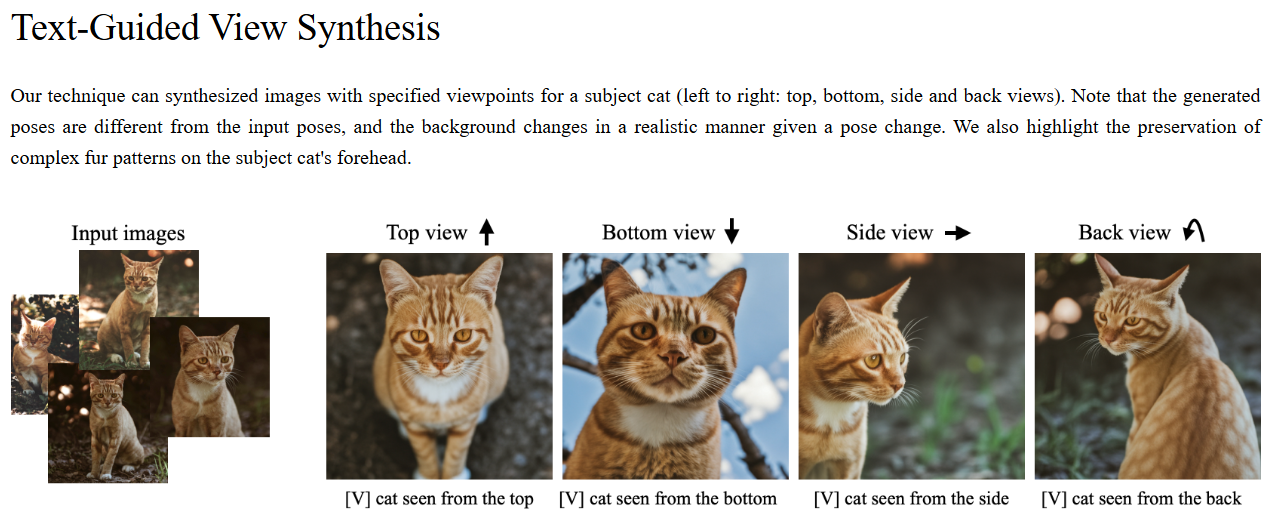
\includegraphics[width=\linewidth,height=\textheight,keepaspectratio]{images/adv-img-gen/dreambooth-result-3.png}
    \small [Ruiz et al., 2023](https://arxiv.org/abs/2208.12242)
\end{figure}

\framebreak
\begin{figure}
    \centering
    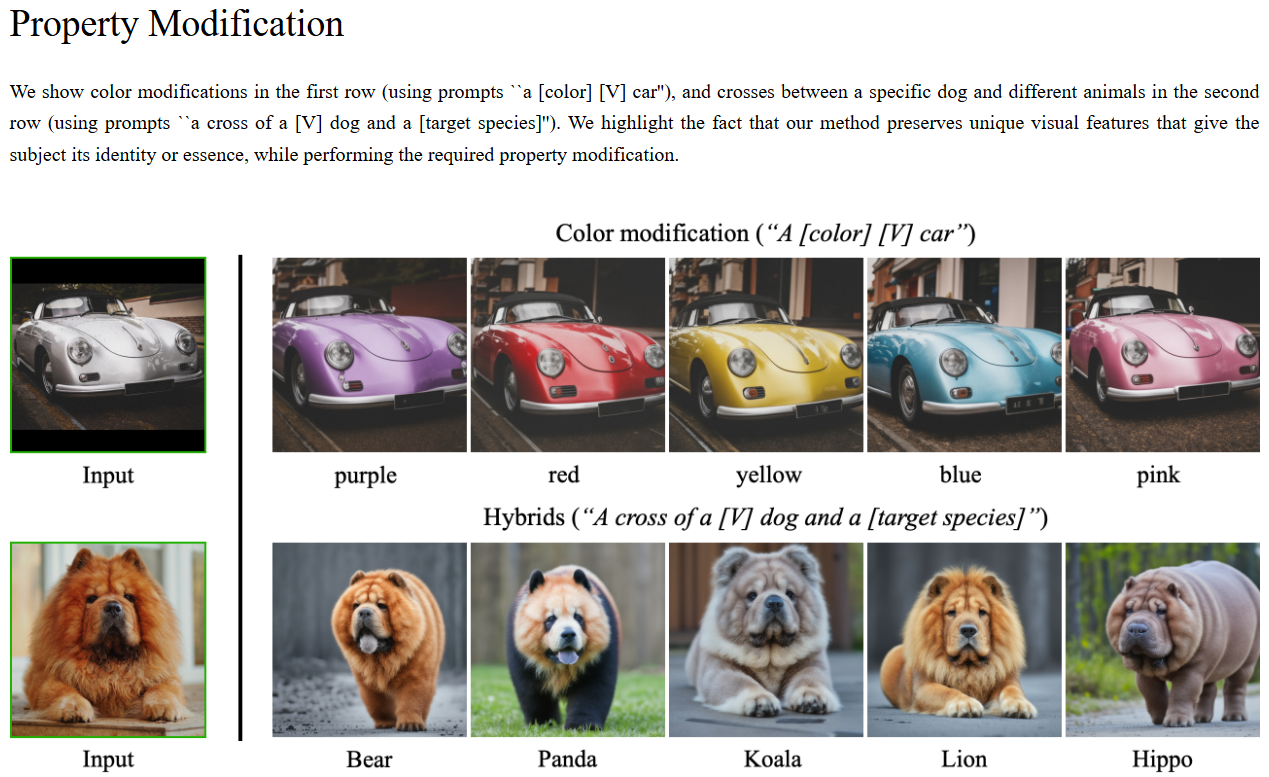
\includegraphics[width=\linewidth,height=\textheight,keepaspectratio]{images/adv-img-gen/dreambooth-result-4.png}
    \small [Ruiz et al., 2023](https://arxiv.org/abs/2208.12242)
\end{figure}

\framebreak
\begin{figure}
    \centering
    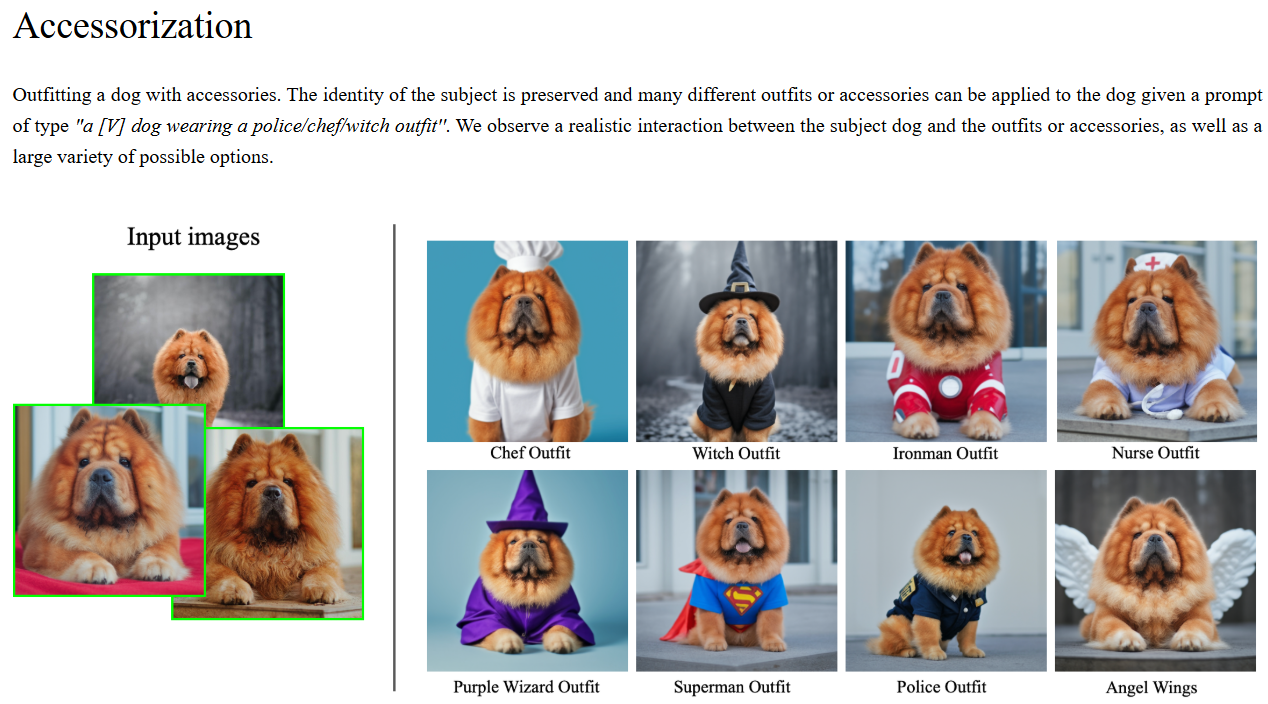
\includegraphics[width=\linewidth,height=\textheight,keepaspectratio]{images/adv-img-gen/dreambooth-result-5.png}
    \small [Ruiz et al., 2023](https://arxiv.org/abs/2208.12242)
\end{figure}
\end{frame}